\documentclass{beamer}
\setbeamertemplate{navigation symbols}{}

\usepackage{amsmath}



\title[Collective SRL with ML]{Collective Semantic Role Labelling with Markov Logic}
\author[Riedel and Meza]{Sebastian Riedel \qquad Ivan Meza-Ruiz}
\institute[ICCS, UoE]{Institute for Communicating and Collaborative Systems\\
  School of Informatics\\
  University of Edinburgh\\
  {\tt\{S.R.Riedel,I.V.Meza-Ruiz\}@sms.ed.ac.uk} }
\date{August 16th, 2008}

\usetheme{Madrid}

\begin{document}
\begin{frame}
\titlepage
\end{frame}

\begin{frame}
    \frametitle{ Our intuitions of the SRL task}
    \begin{center}
        \includegraphics[scale=.70]{example-2}
    \end{center}
   
    \begin{itemize}
        \item A predicate can have at most one argument of a proper argument role.
    \end{itemize}
\end{frame}


\begin{frame}
    \frametitle{ Our intuitions of the SRL task}
    \begin{center}
        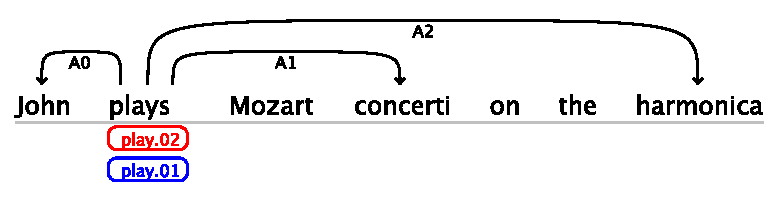
\includegraphics[scale=.70]{example-1}
    \end{center}

    \begin{itemize}
        \item Sense of a verbe correlates with the arguments roles of a verb.
    \end{itemize}
\end{frame}

\begin{frame}
    \frametitle{ Our intuitions of the SRL task}
    \begin{center}
        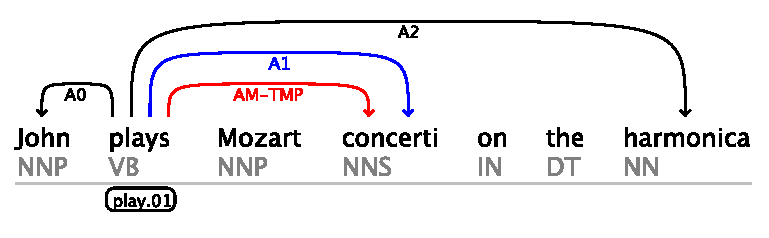
\includegraphics[scale=.70]{example-3}
    \end{center}

    \begin{itemize}
                    \item Semantic role labels correlates with their POS tags
    \end{itemize}
\end{frame}

\begin{frame}
    \frametitle{Capturing our intuitions}
    
    \begin{itemize}
        \item Local: classifier, easy to do
        \item Global: pipeline, reranking, ILP, approximate heuristic search, harder to engineer
        \item Markov Logic (other, Statistical relational learning), easy to capture intuition
    \end{itemize}
\end{frame}

\begin{frame}
\tableofcontents
\end{frame}

\section{Markov Logic}

\begin{frame}
 \frametitle{Markov Logic}
 \begin{itemize}
 \item Combines of FOL and Markov Networks
 \item Defines a log-linear distribution over possible worlds
 \item Uses weigthed FOL formulae 
 \end{itemize}
\end{frame}

\begin{frame}
    \frametitle{Vocabulary}
    The vocabulary consists of:
    \begin{itemize}
        \item \emph{Constants} represent objects of the domain (e.g., Haag, VB,
            1, 2, 3, \ldots)
        \item \emph{Predicates} represent relations over the objects
    \end{itemize}
    \bigskip
    There are two types of predicates: Observable and hidden. \\Some of the observable predicates are:
    \begin{itemize}
    \item \emph{word/2}, \emph{word(1,Haag)}
    \item \emph{pos/2},  \emph{pos(1,NNP)}
    \item \emph{path/3}, \emph{path(2,1,$->$)}
    \end{itemize}
    
\end{frame}

\begin{frame}
    \frametitle{Hidden predicates}
\begin{figure}
\begin{center}
   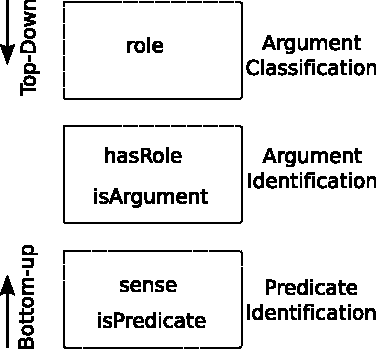
\includegraphics[scale=.70]{TaskArchitecture}
\end{center}
\caption{Hidden predicates}
\label{fig:task}
\end{figure}

Input : \[\{word(1,Mr.),word(2,Haag), word(3,plays), word(4,elianti), \ldots \}\]
Output : \[\{isPredicate(3), sense(3,02), isArg(2), hasRole(3,2), role(3,2,A0), \ldots \}\]

\end{frame}

\section{Modelling}

\begin{frame}
    \frametitle{Formulae}
    We use formulae to capture statements about the world.

    \begin{itemize}
        \item Local formulae
        \bigskip
        \item Global formulae
    \end{itemize}
\end{frame}


\begin{frame}
    \frametitle{Formulae}

    Structural constraints ensure the possible world is valid

    \begin{center}
        \includegraphics[scale=.70]{example-2}
    \end{center}
 
 \begin{eqnarray*}
    role(p,a,r_1) \wedge r_1 \neq r_2 \Rightarrow \neg role(p,a,r_2) 
 \end{eqnarray*}


\end{frame}


\begin{frame}
    \frametitle{Formulae}
    Hard constraints about the nature of the task
    \begin{center}
        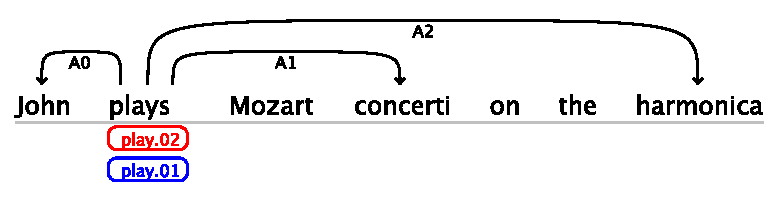
\includegraphics[scale=.70]{example-1}
    \end{center}

 \begin{eqnarray*}
 &role\left(p,a_{1},r\right)\wedge \neg mod\left(r\right)\wedge a_{1}\neq a_{2}  \Rightarrow\\
  & \neg role\left(p,a_{2},r\right)
 \end{eqnarray*}


\end{frame}


\begin{frame}
    \frametitle{Formulae}
    Soft constraints which depend on the configuration of the predicates 
    \begin{center}
        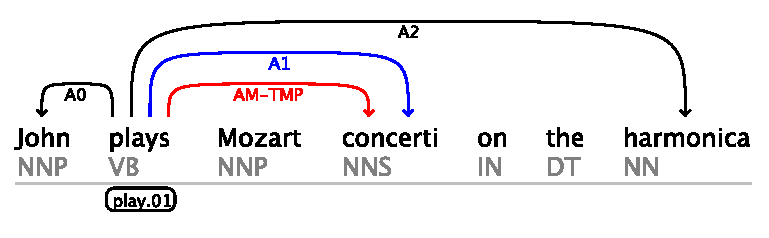
\includegraphics[scale=.70]{example-3}
    \end{center}

 \begin{eqnarray*}
  & lemma(p,+l) \wedge ppos(a,+p)  \\
  & \wedge hasRole(p,a)  \Rightarrow sense(p,+f) 
 \end{eqnarray*}
\end{frame}


\begin{frame}
    \frametitle{Markov Logic Network}
    A set a weighted formulae is call an Markov Logic Network (MLN). 
    An MLN defines a Markov Network where:
    \begin{itemize}
    \item There is a binary node for each ground atom (e.g., \emph{role(2,1,A1)}.)
    \item There is a factor for each assignment of the free variable of each formulae. 
    \end{itemize}

%\begin{eqnarray*}
%\prob\left(\y\right)=\frac{1}{Z}\exp\left(
%\sum_{\left(\phi,w\right)\in M} w
%\sum_{\boldc\in C^{n_{\phi}}}f_{\boldc}^{\phi}\left(\y\right)
%\right)
%\end{eqnarray*}

\end{frame}

\section{Experiments}
\begin{frame}
    \frametitle{Experiments}

    \begin{itemize}
    \item Whole model: includes all the rules we come up with.
    \item Bottom-Up model: discard top-down rules, it resembles a pipeline where candidates are picked by latter module.
    \item Top-down model: discard bottom-up rules, it resembles a pipeline where candidates are picked by earlier module.
    \item Isolated: discard bottom-up and top-down rules.
    \item Structural: discard the soft global rules.
    \end{itemize}
\end{frame}

\begin{frame}
    \frametitle{Results}

\begin{table}
\begin{center}
\small
\begin{tabular}{|l|l|l|c|c|}\hline
Model                & WSJ                & Brown              & Train & Test\\
                     &                    &                    & Time & Time\\\hline\hline
Full         & $75.72\%$          & $\mathbf{65.38}\%$ & 25h & 24m\\\hline
Up           & $\mathbf{76.96\%}$ & $63.86\%$          & 11h & 14m\\\hline
Down         & $73.48\%$          & $59.34\%$          & 22h & 23m\\\hline
Isolated     & $60.49\%$          & $48.12\%$          & 11h & 14m\\\hline
Structural   & $74.93\%$          & $64.23\%$          & 22h & 33m\\\hline   
\end{tabular}
\caption{F-scores for different models.}
\label{tbl:results}
\normalsize
\end{center}
\end{table}
\end{frame}

\section{Conclusion}
\begin{frame}
    \frametitle{Conclusions}

    \begin{itemize}
    \item This network achieves the second best semantic F-
scores in the Open Track of the CoNLL shared task for only SRL.
    \bigskip
    \item The bottom-up model reaches a better performance.
    \end{itemize}
\end{frame}

\begin{frame}
    \frametitle{Pointers}

    \begin{itemize}
    \item Implementation of ML:\\ \texttt{http://thebeast.googlecode.com/}
    \bigskip 
    \item Models and scripts:\\ \texttt{http://thebeast.googlecode.com/svn/mlns/conll08/}
    \end{itemize}
\end{frame}



\end{document}
